\chapter{Mise en équation}

\section{La couche limite}

\begin{figure}[h!]
	\centering
	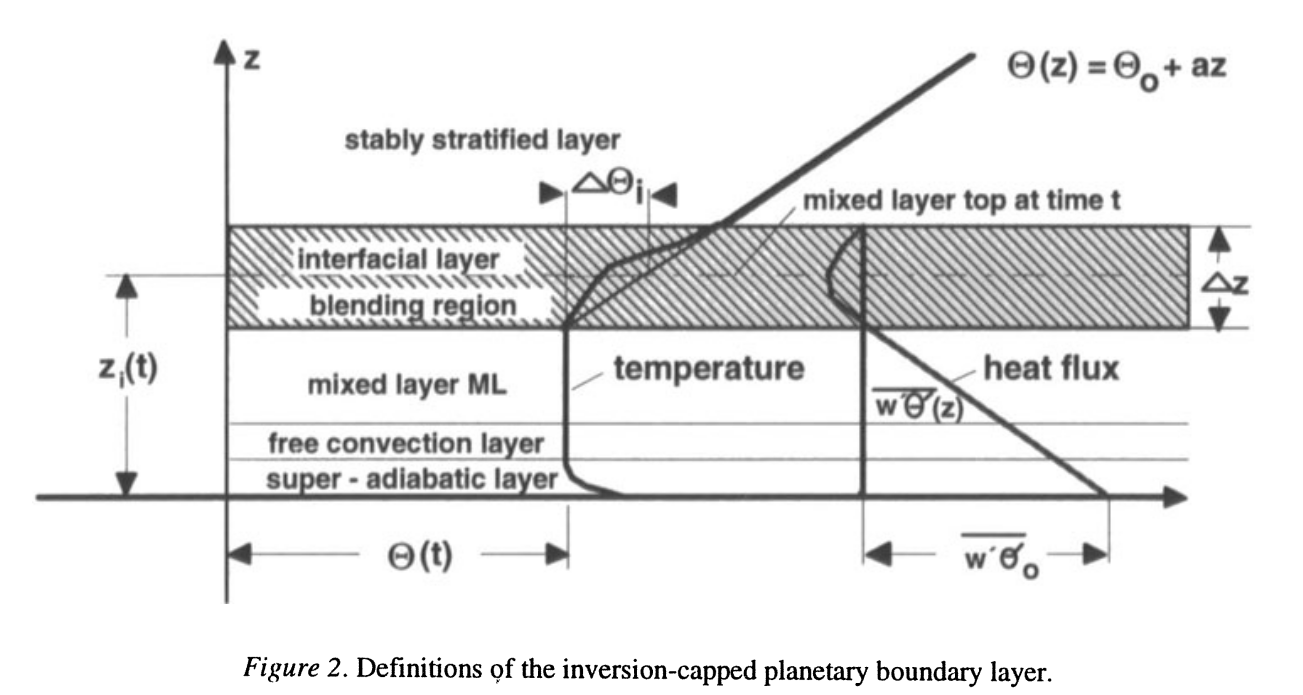
\includegraphics[width=0.7\linewidth]{FIGURES/PBL}
	\caption{}
	\label{fig:pbl}
\end{figure}


\section{Rayleigh-Bénard convection}
Décrit la convection naturelle. Fluide entre deux plaque séparée d'une distance $h$ à température fixes $T_b$ et $T_h$ avec $Th > Tb$. 

\begin{figure}[h!]
	\centering
	\includegraphics[width=0.4\linewidth]{../../../../RB}
	\caption{}
	\label{fig:rb}
\end{figure}

\subsection{Mise en équation du problème}
\paragraph{Incompressibilité} On considère le fluide comme incompressible; écoulement avec des vitesses inférieurs à Mach 0.3 donne une faibel déformation dû  la vitesse. 
\begin{equation}
	\nabla \cdot V = 0
\end{equation}

\paragraph{Quantité de mouvement} Conservation de la qtité de mvt s'écrit :
\begin{equation}
	\rho_0 \left(\partial_t + V \cdot \nabla) V \right)= - \nabla \rho + \eta \nabla ^2 V + \rho g 
\end{equation}
avec $\rho_0$ la masse volumique dans la situation de référence, $\eta$ la viscosité dynamique. 
Avec l'approximation de Boussinesq ($\delta \rho << \rho_0$) : $\rho = \rho_0 (1- \alpha(T-T_0))$ où $\alpha$  coefficient de dilatation thermique. 
 
\begin{equation}
	\left(\partial_t + V \cdot \nabla \right) V = - \frac{1}{\rho_0} \nabla p + \nu \nabla ^2 V + \left( 1-\alpha(T-T_0)\right) g 
\end{equation}
Et $\nu = \eta / \rho$ est la viscosité cinématique. 

\paragraph{Equation de la chaleur}
\begin{equation}
	\partial_t T + V \cdot \nabla T = \kappa \Delta T
\end{equation}
A l'équilibre 
\begin{equation}
	\left(\partial_t + V \cdot \nabla \right) V = 0 = - \frac{1}{\rho_0} \nabla p_s + \nu \nabla ^2 V + g 
\end{equation}
On peut perturber le système avec $p = p_s + p'$, et $T = T_c(z) + \theta(x,z,t)$ 

Le problème s'écrit donc
\begin{equation}
	\begin{cases}
	\nabla \cdot V = 0 \\
	\frac{1}{P_r}\left(\partial_t + V \cdot \nabla \right) V = - \nabla p + \nabla ^2 V + \theta e_z \\	
	\left(\partial_t + V \cdot \nabla\right) \theta = R_a v_z + \Delta \theta
\end{cases}
\end{equation}

\subsection{Stabilité}

On s'intéresse au cas de Rayleigh-Bénard avec aucune dépendance en $y$, donc que $\partial_y = 0$ et $v=0$. 
fluide incompressible (expliquer pk?)\\
Système étudié décrit par les équations de Boussinesq : 

Ce pb est étudié pour Rayleigh-Bénard = instabilité de convection. On trouve un point de bifurcation $\propto \Delta t$, cas pour les rouleaux plus compliqué car instabilité de vent/ cisaillement ? étude par \cite{liuAnalyticalModelRoll2009}.

\section{Etude de stabilité} Etude de l'effet d'une perturbation sur un état de base. Connaitres les états et les bifurcations possibles. Le souci c'est la complexité du système dynamique étudié. \\

\subsection{Obtention des EDO d'un système dynamique}
Étude mené sur des système dynamiques = EDO
 \begin{equation}
 	\label{eq:EDOdyn}
 	\dot X = F(X, r, t) 
 \end{equation}
 mais les équations physiques, notamment de la dynamique, sous formes d'EDP 
 \begin{equation}
 	\label{eq:EDPphys}
 	\frac{\partial V}{\partial t} = \mathcal L(V) + \mathcal{N} (V)
\end{equation}
 où $\mathcal L$ est un opérateur linéaire. On fait des études autour d'une situation de base connue. $\mathcal{L}$ fait apparaitre les cohérence spatiales, retroactions linéaires dans ses modes propres. \\
 On cherche des solutions à variables séparées et si $\mathcal{L}$ peut etre auto-adjoint c'est chouette :) \\
 Le problème apres c'est plus de traiter $\mathcal{N}$ mais avec dvp de Taylor on peut se ramener à une équatio nde la dynamique. \\
 \textbf{Objectif ? } Est ce que ça peut etre un objectif de mettre le problème sous forme de problème dynamique? \\

\subsection{Cas de la convection de Rayleigh-Bénard}

% Study of stability of the Rayligh Benard convection => Rayleigh number to decide when the convection begins. Rolls is basicely the same but with wind ? so mabe try to do the same 
% Study of unstabilities that lead to rolls= expected basic state of hurricane BL (\cite{foster_why_2005}. )
